\documentclass{article}
\usepackage{graphicx}
\usepackage[T1]{fontenc}
\usepackage{hyperref}
\usepackage{caption}
\usepackage{times}
\usepackage{amsmath}
\usepackage{lipsum}
\usepackage[margin=1.3in]{geometry}


\title{Kategorik Veri Çözümlemesi}
\author{Ramazan Erduran}
\date{May 2023}

\begin{document}
\begin{titlepage}
    \begin{center}
        
\includegraphics[width=0.5\textwidth]{Imgs/hacettepe_logo.png}
        
        \vspace*{1cm}
        \Huge
        \textbf{Kategorik Veri Çözümlemesi Dönem Ödevi}

        \vfill
        
        \Large
        \textit{Ramazan Erduran ~ 21821809 \\
        İlkay Şafak Baytar ~ 21935712 \\
        İhsan Tutak ~ 21822178
        }\\
        
        \vfill
        Hacettepe Üniversitesi \\
        İstatistik \\
        
    \end{center}
\end{titlepage}

\newpage

\tableofcontents
\clearpage

\section{Araştırmanın Hakkında}
\subsection{Araştırmanın Başlığı}
Fen Fakültesi Öğrencilerinin İkili İlişkilerinin İncelenmesi.

\subsection{Araştırmanın Amacı}

\subsection{Örnekleme Planlaması}
Araştırmalar sonucunda Hacettepe Üniversitesi'nin yayınladığı bilgilere dayanarak öğrenci, öğretim üyesi oranı, Tablo. \ref{tab:Öğrenci:Öğretim Üyesi Oranları} 'deki veriler bulunmuştur.

\begin{table}[h]
    \centering
    \caption{Öğrenci:Öğretim Üyesi Oranları}
    \label{tab:Öğrenci:Öğretim Üyesi Oranları}

    \begin{tabular}{|p{2.1cm}|p{2.1cm}|p{2.1cm}|p{2.1cm}|p{2.1cm}|}
        \hline
         & Tıp ve Sağlık & Fen ve Mühendislik & Sosyal ve Beşeri Bilimler & Toplam \\
        \hline
        Öğretim Üyesi'ne Oranı & 16:1 & 35:1 & 46:1 & 30:1 \\
        \hline
        Öğretim Elemanı'na Oranı & 6:1 & 22:1 & 23:1 & 14:1 \\
        \hline
    \end{tabular}
    \caption*{\footnotesize Kaynak:\url{https://www.hacettepe.edu.tr/ogretim/sayilarla_ogretim}}
\end{table}

Ayrıca her bölümün kendi sayfasında öğretim üyelerinin kesin sayıları olduğundan toplam öğrenci sayısının hesaplanmasında belirtilen varsayımlar kullanılmıştır.

\begin{table}[h]
    \centering
    \caption{Bölüm Bazlı Akademik Personel Sayısı}
    \label{tab:Bölüm Bazlı Veriler}
    
    \begin{tabular}{|c|c|c|}
         \hline
         Bölüm & Öğretim Elemanı Sayısı & Tabaka Ağırlığı\\
         \hline
         İstatistik & 26 & 0.13 \\
         Aktüerya & 6 & 0.03 \\
         Matematik & 41 & 0.20 \\
         Kimya & 51 & 0.25 \\
         Biyoloji & 81 & 0.39 \\
         \hline
         Toplam & 205 & 1.00 \\
         \hline
    \end{tabular}
\end{table}

\clearpage

\begin{table}[h]
    \centering
    \caption{Bölümlere Göre Öğrenci Sayıları}
    \label{tab:Bölüm bazlı öğrenci sayıları}
    \begin{tabular}{|c|c|}
        \hline
        Bölüm & Öğrenci Sayısı\\
        \hline
        İsatistik & 572 \\
        Aktüerya & 132 \\
        Matematik & 902 \\
        Kimya & 1122 \\
        Biyoloji & 1782 \\
        \hline
        Toplam & 4510 \\
        \hline
    \end{tabular}
\end{table}

Tablo \ref{tab:Bölüm bazlı öğrenci sayıları}'deki öğrenci sayıları, Tablo \ref{tab:Öğrenci:Öğretim Üyesi Oranları} ve Tablo \ref{tab:Bölüm Bazlı Veriler}'den hareketle hesaplanmıştır. 

\vspace{10pt}
\section{Örnekleme Planlaması}
Tablo \ref{tab:Bölüm bazlı öğrenci sayıları}'den hareketle aşağıdaki formül uygulanarak örneklem sayısı elde edilmiştir:
$$
n = N \times \frac{Z^2 \times p \times (1-p)}{d^2 \times (N-1) \times Z^2 \times p \times (1-p)}
$$

Formülde kullanılan parametreler;
\begin{itemize}
    \item Z = 1.96 (\%95 Güven Düzeyinde)
    \item N = 4510
    \item d = 10
    \item p = 0.5
\end{itemize} şeklindedir. Formül uygulandıktan sonra $n=68.34 \approx 68$ olarak bulunmuştur. Bulunan örneklem sayısı bölümlerin tabakalı ağırlıklarına göre dağıtıldığında toplanması gerekilen örneklem sayısı Tablo \ref{tab:ağırlıklandırılmış örneklem}'deki gibi elde edilmiştir.

Bu örnekleme planı ışığında yapılan ankete \href{https://docs.google.com/forms/d/e/1FAIpQLSf7CBA1tg89lFSdAl9VRSa4vjmv8COCJtRDvQmYa0n0l72JUA/viewform?usp=sf_link}{buradan} ve kaynak \ref{form} 'den ulaşılabilir. 

\begin{table}[h]
    \centering
    \caption{Bölümlere Göre Örneklem Sayısı}
    \label{tab:ağırlıklandırılmış örneklem}
    \begin{tabular}{|c|c|}
         \hline
         Bölüm & Örneklem Sayısı \\
         \hline
         İstatistik & 9 \\
         Aktüerya & 2 \\
         Matematik & 14 \\
         Kimya & 17 \\
         Biyoloji & 25 \\
         \hline
         Toplam & 68 \\
         \hline
    \end{tabular}
\end{table}

\clearpage

\begin{twocolumn}
\section{Çözümlemeler}
\subsection{Tek Değişkenli Görselleştirme}

    \begin{figure}[htbp]
        \centering
        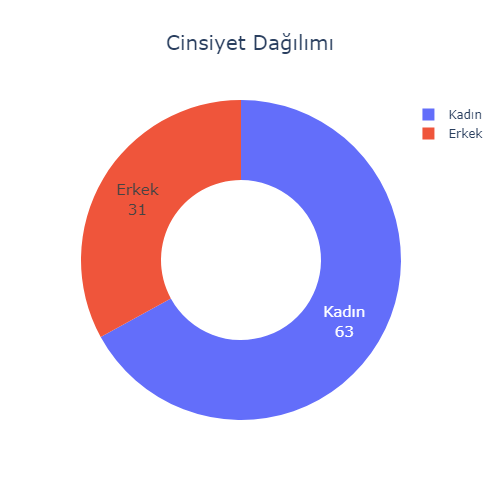
\includegraphics[width=0.5\textwidth]{Imgs/soru1.png}
        \caption{Cinsiyet}
        \label{soru1}
    \end{figure}    
Resim \ref{soru1}'den hareketle katılımcılardan 63 tanesi kadınken 31 tanesi ise erkek olduğu çıkarımı yapılmaktadır.

    \begin{figure}[htbp]
        \centering
        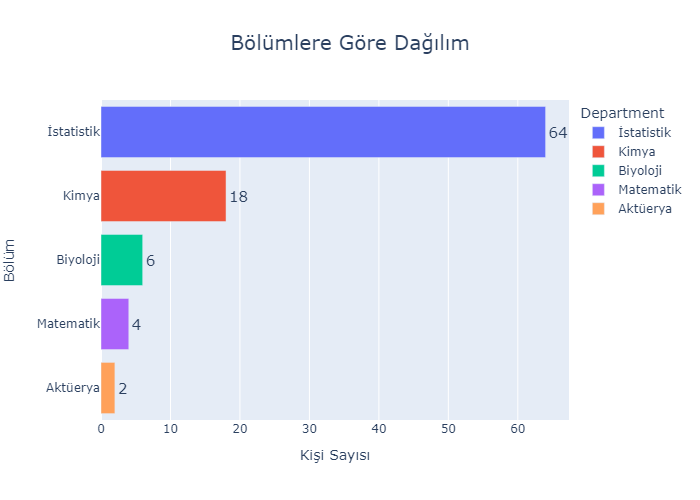
\includegraphics[width=0.5\textwidth]{Imgs/soru2-2.png}
        \caption{Bölüm}
        \label{soru2}
    \end{figure}
Resim \ref{soru2}'den hareketle, 64 katılımcı İstatistik, 18 katılımcı Kimya, 6 Katılımcı Biyoloji, 4 katılımcı Matematik ve 2 katılımcı ise Aktüerya bölümlerinde okumakatadır.

    \begin{figure}[htbp]
        \centering
        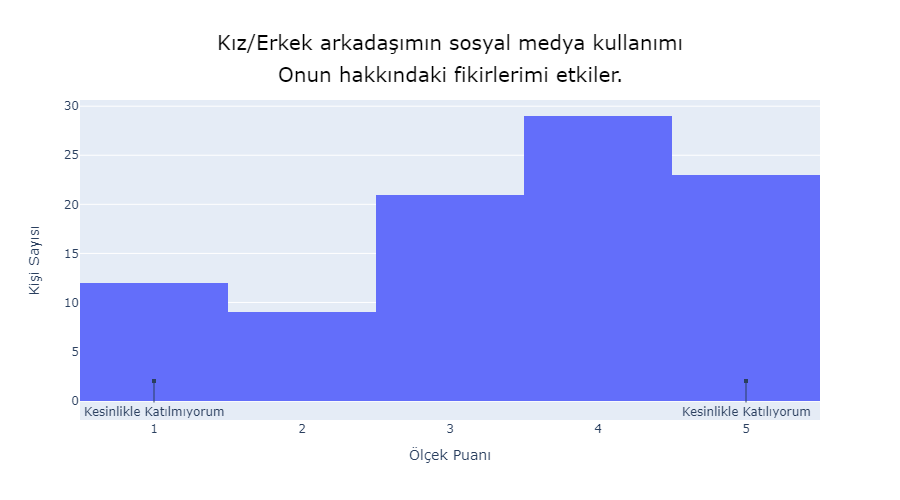
\includegraphics[width=0.5\textwidth]{Imgs/likert1.png}
        \caption{Likert Ölçek Sorusu: 1}
        \label{likert1}
    \end{figure}
Resim \ref{likert1}'den hareketle \textit{"Kız/Erkek arkadaşımın  sosyal medya kullanımı onun hakkındaki fikirlerimi etkiler."} fikrine ağırlıkça katılımcılar katılma eğilimi göstermektedirler.

    \begin{figure}[htbp]
        \centering
        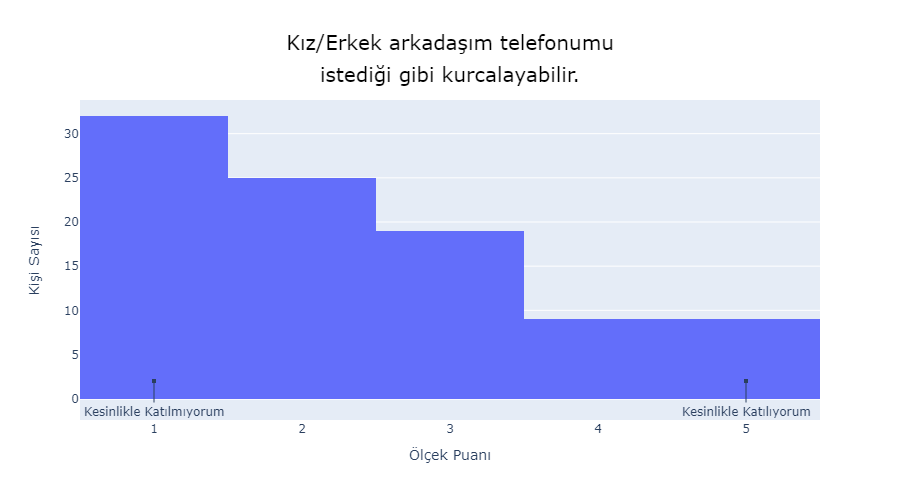
\includegraphics[width=0.5\textwidth]{Imgs/likert2.png}
        \caption{Likert Ölçek Sorusu: 2}
        \label{likert2}
    \end{figure}
Resim \ref{likert2}'den hareketle \textit{"Kız/Erkek arkadaşım telefonumu istediği gibi kurcalayabilir."} önergesine katılımcılarımız ağırlıklı olarak kesinlikle katılmıyorum şeklinde yanıt vermişlerdir.

    \begin{figure}[htbp]
        \centering
        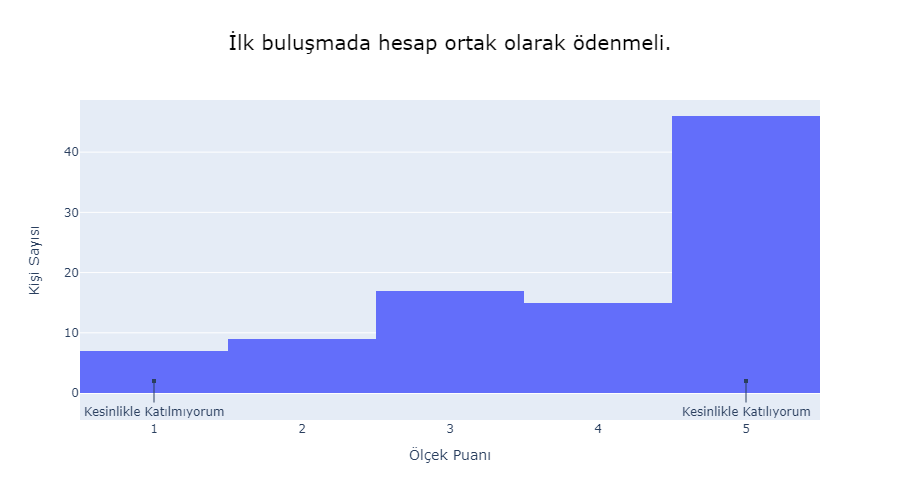
\includegraphics[width=0.5\textwidth]{Imgs/likert3.png}
        \caption{Likert Ölçek Sorusu: 3}
        \label{likert3}
    \end{figure}
Resim \ref{likert3}'den hareketle \textit{"İlk buluşmada hesap ortak olarak ödenmeli."} önergesine katılımcılar çok yüksek bir sayıyla kesinlikle katılıyorum seçeneğini seçmişler.

\clearpage
    \begin{figure}[htbp]
        \centering
        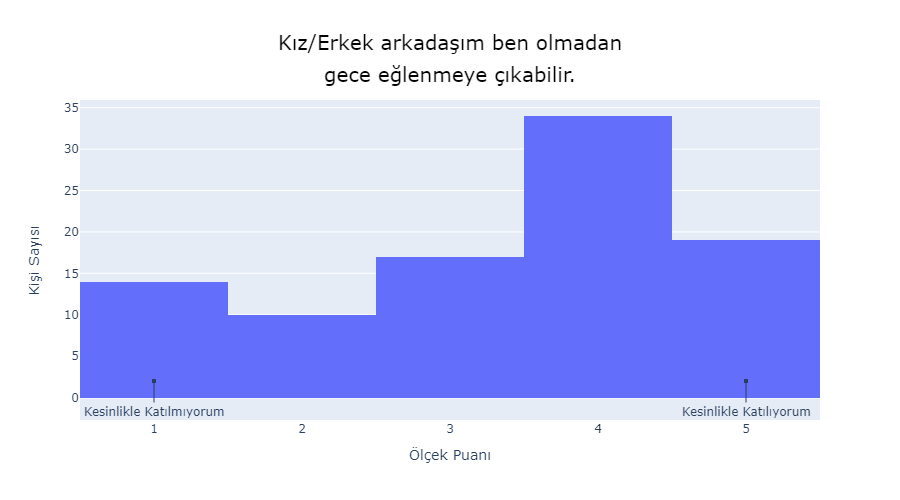
\includegraphics[width=0.5\textwidth]{Imgs/likert4.png}
        \caption{Likert Ölçek Sorusu: 4}
        \label{likert4}
    \end{figure}
Resim \ref{likert4}'den hareketle \textit{"Kız/Erkek arkadaşım ben olmadan gece eğlenmeye çıkabilir."} önergesine katılımcıların çoğu katıldıkları yönünde işaretleme yapmaktadırlar.

    \begin{figure}[htbp]
        \centering
        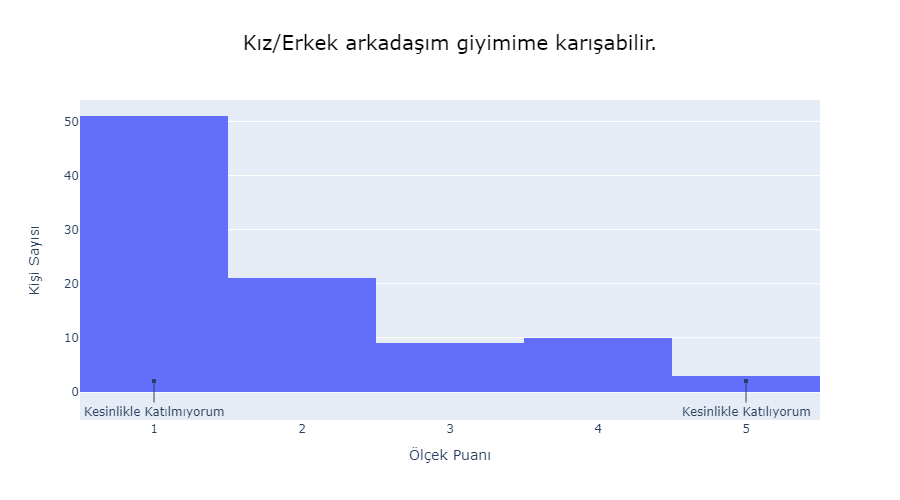
\includegraphics[width=0.5\textwidth]{Imgs/likert5.png}
        \caption{Likert Ölçek Sorusu: 5}
        \label{likert5}
    \end{figure}
Resim \ref{likert5}'den hareketle \textit{"Kız/Erkek arkadaşım giyimime karışabilir."} önergesine yüksek bir çoğunlukla katılımcılar "Kesinlikle Katılmıyorum" şeklinde yanıtlamaktadırlar.

    \begin{figure}[htbp]
        \centering
        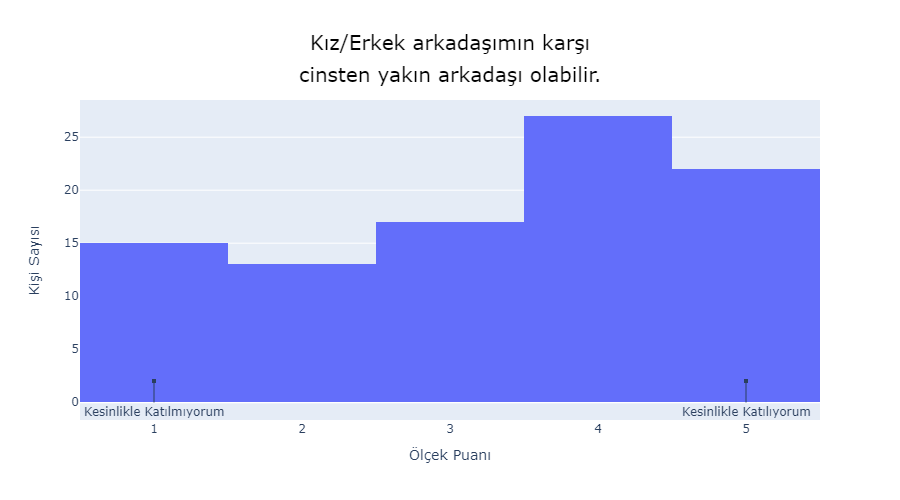
\includegraphics[width=0.5\textwidth]{Imgs/likert6.png}
        \caption{Likert Ölçek Sorusu: 6}
        \label{likert6}
    \end{figure}
Resim \ref{likert6}'dan hareketle \textit{"Kız/Erkek arkadaşımın karşı cinsten yakın arkadaşı olabilir."} önergesine verilen yanıtlar biraz daha simetrik dağılmaya çalışmış olsa da ortalama olarak katılımcılar katıldıkları yönde işaretleme yapmaktadır.

    \begin{figure}[htbp]
        \centering
        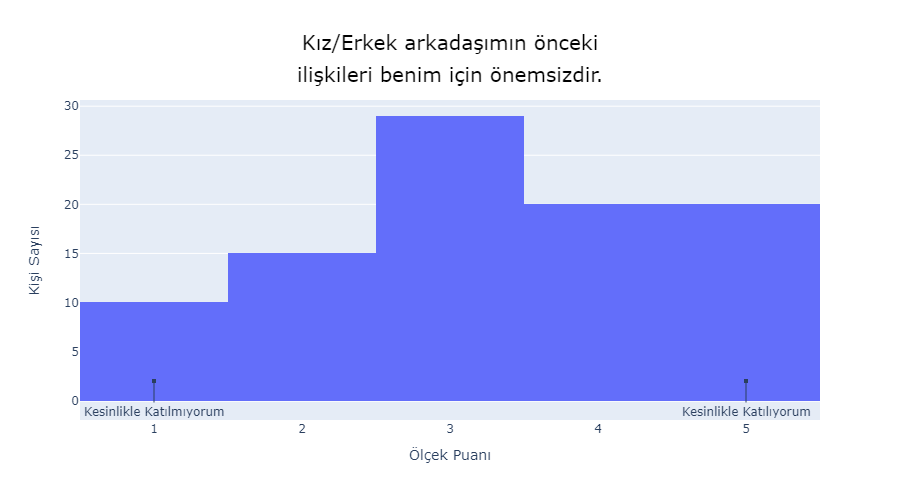
\includegraphics[width=0.5\textwidth]{Imgs/likert7.png}
        \caption{Likert Ölçek Sorusu: 7}
        \label{likert7}
    \end{figure}
Resim \ref{likert7}'dan hareketle \textit{"Kız/Erkek arkadaşımın önceki ilişkileri benim için önemsizdir."} önergesine katılımcılar kararsız olarak yanıt vermektedirler. Ancak dağılım sağ kolunda (önergeye katılan taraf), sol kolundan (önergeye katılmayan taraf) daha fazla katılımcı içermektedir.

    \begin{figure}[htbp]
        \centering
        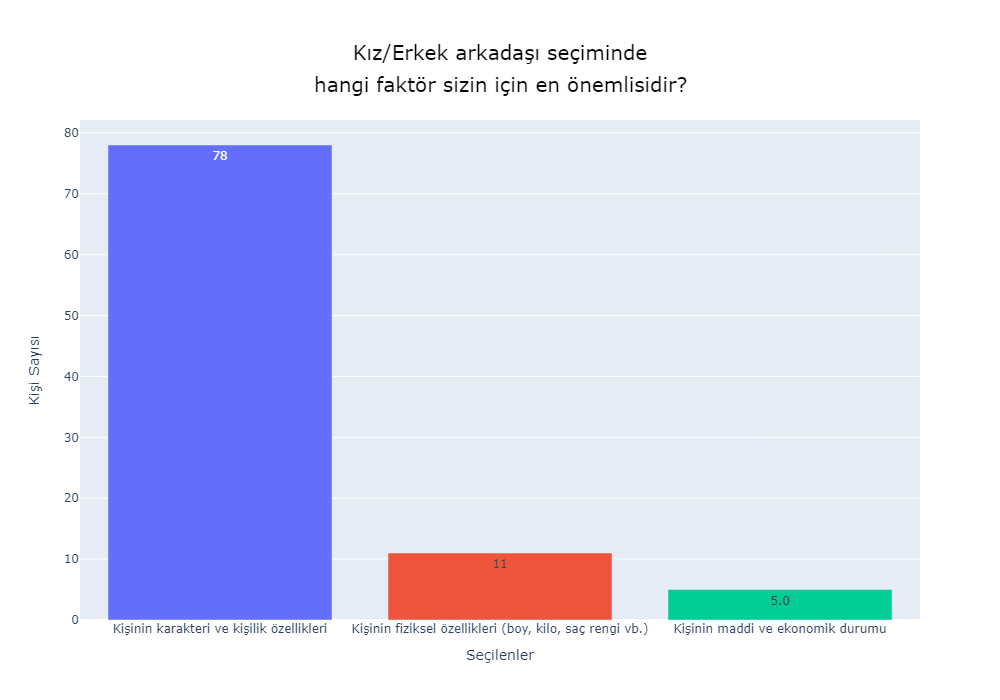
\includegraphics[width=0.5\textwidth]{Imgs/soru10.png}
        \caption{En Önemli Kriter Seçimi}
        \label{soru10}
    \end{figure}
Resim \ref{soru10}'den hareketle \textit{"Kız/Erkek arkadaşı seçiminde hangi faktör sizin için en önemlisidir?"} sorusunun verilen yanıtların büyük bir çoğunluğu kişinin karakteri yönünde olurken "Kişinin eğitim seviyesi ve akademik başarısı" seçeneği ile "Kişinin ailevi durumu ve aile geçmişi" seçeneği kimse tarafından seçilmemektedir.

\clearpage
    \begin{figure}[htbp]
        \centering
        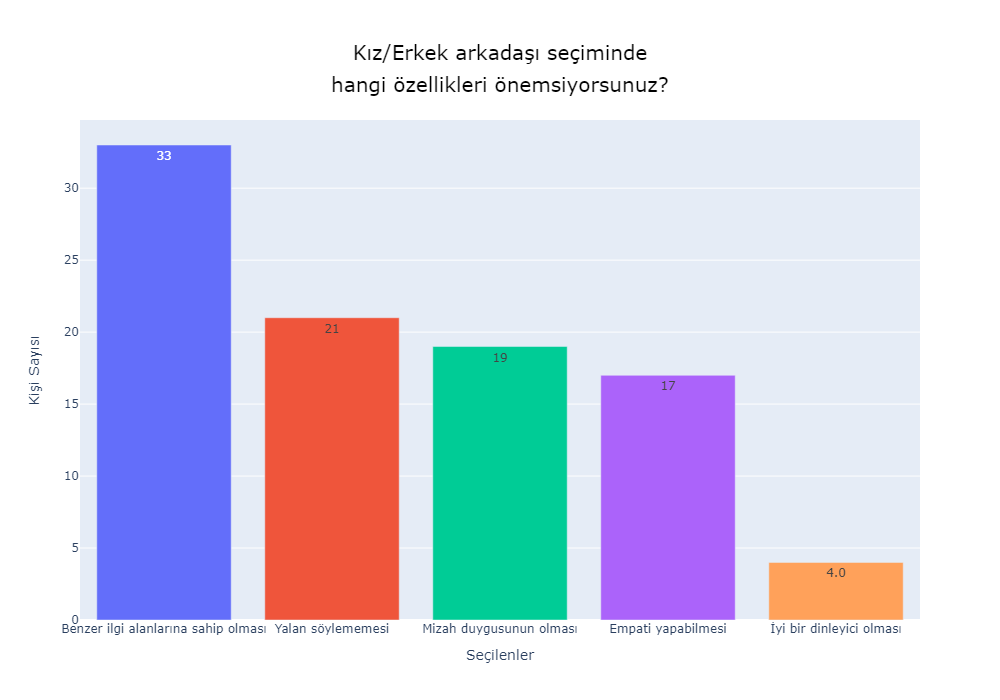
\includegraphics[width=0.5\textwidth]{Imgs/soru11.png}
        \caption{Özellik Seçimi}
        \label{soru11}
    \end{figure}
Resim \ref{soru11}'den hareketle \textit{"Kız/Erkek arkadaşı seçiminde hangi özellikleri önemsiyorsunuz?"} sorusuna verilen yanıtlara bakıldığında tüm seçenekler en az 4 katılımcı tarafından desteklenmiş. Benzer ilgi alanlarına sahip olmayı isteyen katılımcı sayısı çoğunlukta iken, en az desteği gören seçenek "İyi bir dinleyici olması" seçeneği olmaktadır.

    \begin{figure}[htbp]
        \centering
        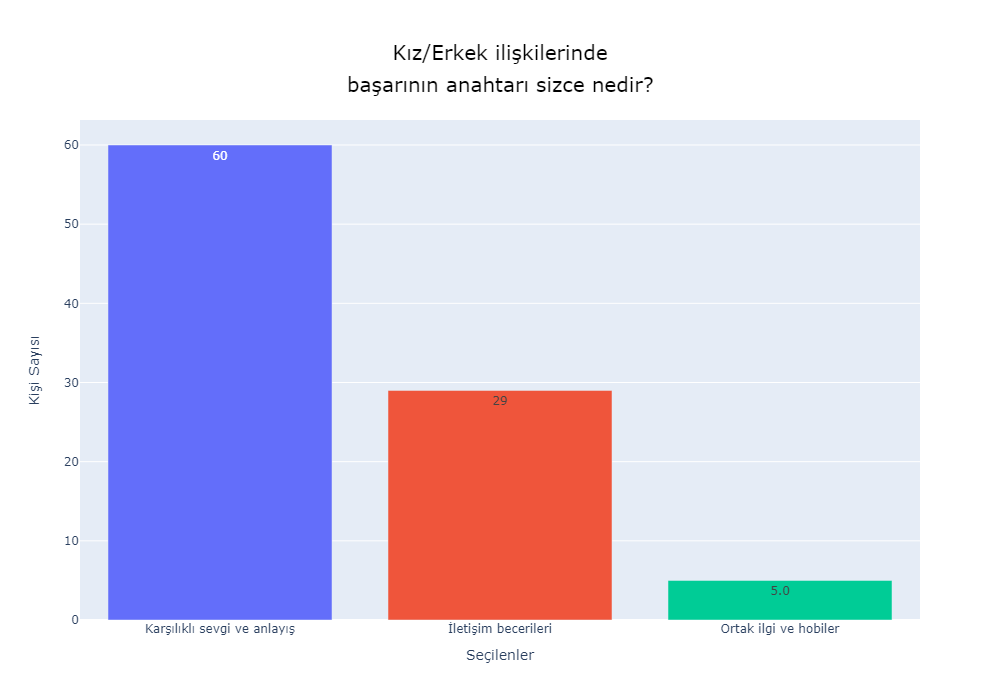
\includegraphics[width=0.5\textwidth]{Imgs/soru12.png}
        \caption{Başarının Anahtarı}
        \label{soru12}
    \end{figure}
Resim \ref{soru12}'den hareketle "Kız/Erkek ilişkilerinde başarının anahtarı sizce nedir?" sorusu için karşılıklı sevgi ve anlayış seçeneği en çok desteği alırken, seçeneklerden biri olan "Romantik jestler ve sürprizler" seçeneği hiçbir katılımcı tarafından destek görmemektedir.

    \begin{figure}[htbp]
        \centering
        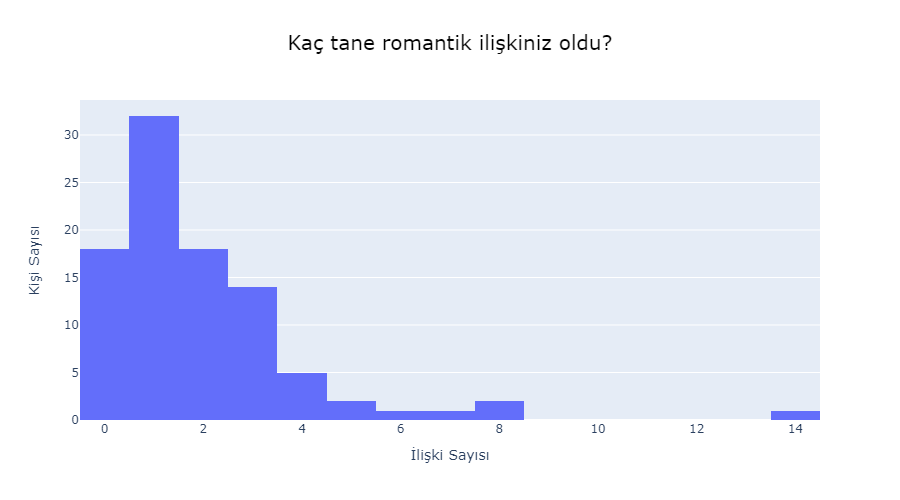
\includegraphics[width=0.5\textwidth]{Imgs/soru13.png}
        \caption{İlişki Sayısı}
        \label{soru13}
    \end{figure}
\newpage
Resim \ref{soru13}'den hareketle \textit{"Kaç tane romantik ilişkiniz oldu."} sorusuna verilen yanıtların dağılımı incelendiğinde;
\begin{enumerate}
    \item Ortalama yanıt 1-2 adet civarındadır.
    \item Soruya verilen yanıtların dağılımı sağa çarpık bir dağılım göstermektedir.
    \item Bazı insanlar fazla ilişki sayısına sahiptir ancak insanların çoğunluğu daha az ilişki sayısına sahiptir.
    \item Dağılım sağa çarpık olduğu için medyan ortalama değerden daha düşüktür.
\end{enumerate}
Yorumları yapılmaktadır.

\end{twocolumn}

\onecolumn
\begin{figure}[htbp]
    \centering
    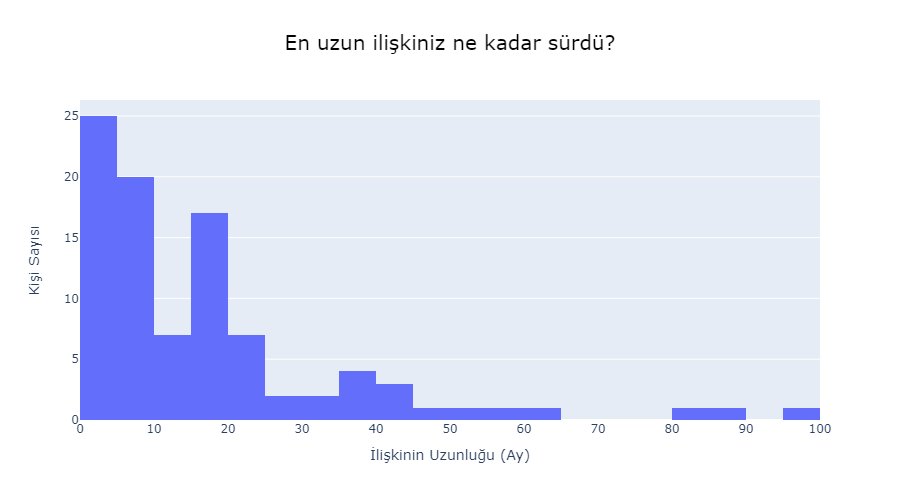
\includegraphics[width=0.8\textwidth]{Imgs/soru14.png}
    \caption{En Uzun İlişki Süresi}
    \label{soru14}
\end{figure}
Resim \ref{soru14}'den hareketle \textit{"En uzun ilişkiniz ne kadar sürdü?"} sorusuna ay bazında verilen yanıtlara bakıldığında, ortalama olarak ilişkilerin 10 ay ve çevresinde sürdüğü ancak 0-5 ay arasında da, 90-100 ay arasında da ilişkisi olan insanların da olduğu yorumu yapılmaktadır. Dağılım sağa çarpık bir dağılımm göstermektedir.

\begin{figure}[htbp]
    \centering
    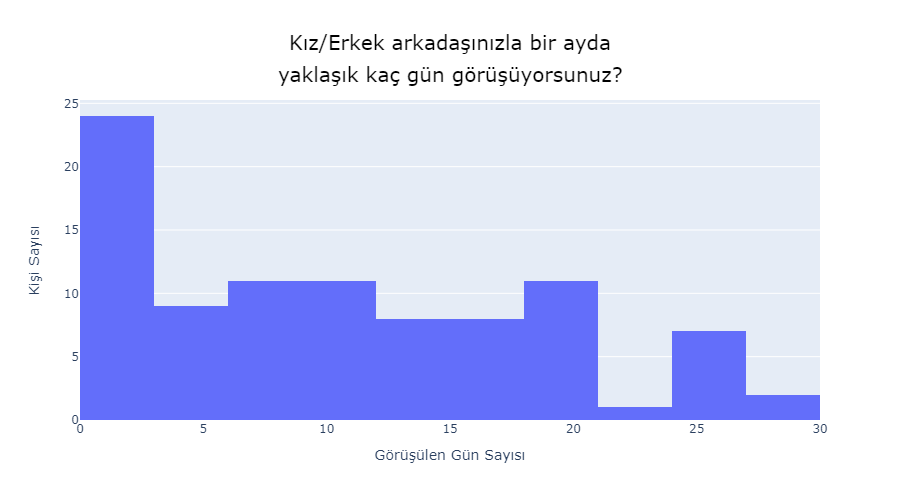
\includegraphics[width=0.8\textwidth]{Imgs/soru15.png}
    \caption{Görüşülen Gün süresi}
    \label{soru15}
\end{figure}
Resim \ref{soru15}'den hareketle \textit{"Kız / Erkek arkadaşınızla bir ayda yaklaşık kaç gün görüşüyorsunuz?"} sorusuna verilen yanıtlarından hareketle, katılımcıların kız/erkek arkadaşlarıyla bir ayda görüştüğü gün hergün (30 gün / 30 gün) olan katılımcılar varken hiç (0 gün/30 gün) olarak seçenler de vardır. Buradan hareketle kız/erkek arkadaşı olmayan katılımcıların varlığından söz edilmektedir.

\clearpage
\vspace{20pt}
\subsection{RxC Çözümlemesi ve Uyum Analizi}
Çözümleme yapılırken değişkenler aşağıdaki gibi belirlenmiştir:
\begin{enumerate}
    \item \textbf{R (Satır Değişkeni)}: Likert 2, Kız/Erkek arkadaşım telefonumu istediği gibi kurcalayabilir.
    \item \textbf{C (Sütun Değişkeni)}: Likert 5, Kız/Erkek arkadaşım giyimime karışabilir.
\end{enumerate}

\begin{figure}[htbp]
    \centering
    \caption{RxC Çapraz Tablosu}
    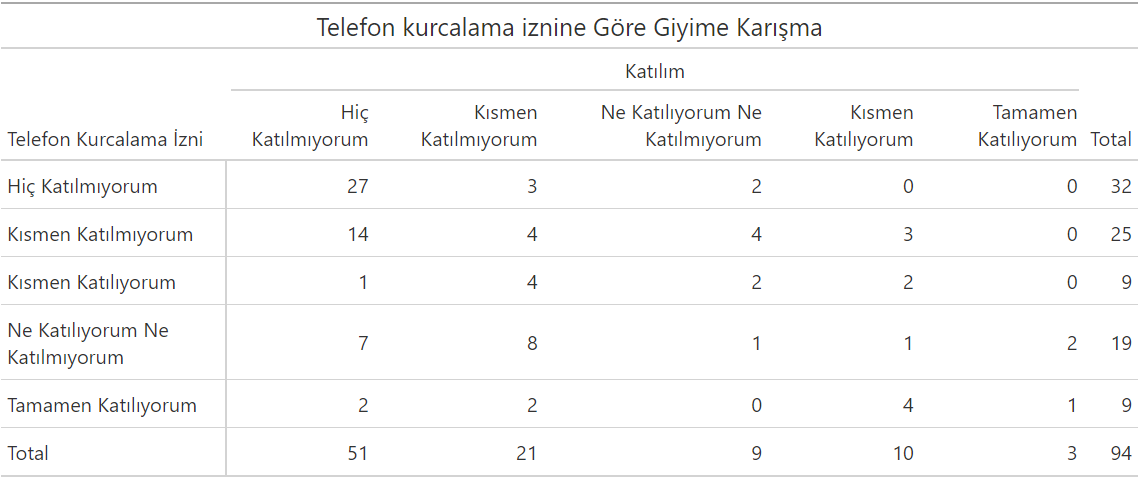
\includegraphics[width=0.8\textwidth]{Imgs/RxC table1.png}
    \label{rxc-table}
\end{figure}

RxC tablosu Tablo \ref{rxc-table}'deki gibi elde edilmiştir.

$H_0:$ Telefon kurcalama izni ile kız/erkek arkadaşın giyime karışması arasında ilişki yoktur.

$H_1:$Telefon kurcalama izni ile kız/erkek arkadaşın giyime karışması arasında ilişki vardır.

\begin{verbatim}
Pearson's Chi-squared test

data:  tablo
X-squared = 45.392, df = 16, p-value = 0.0001208
\end{verbatim}

Yukarıdaki çıktıdan hareketle, p-değeri test için belirlenen hata payı $\alpha=0.05$'ten küçük olduğu için telefona karışma izni ile kız/erkek arkadaşın giyime karışması arasında bir ilişki olduğu \%95 güven düzeyinde söylenebilir.

İlişki katsayısı incelendiğinde:
\begin{enumerate}
    \item X$^2_{Hesap}$ = 45,392
    \item n = 94
    \item $\phi = \sqrt{X^2_{Hesap}/n}=0.6949055$
\end{enumerate}
Olarak elde edilmektedir. Buradan hareketle telefon kurcalama ile kız/erkek arkadaşın giyimine karışması arasında \%70 lik bir ilişki olduğu söylenmektedir.

\clearpage
\begin{figure}[htbp]
    \centering
    \caption{RxC Satır Bazlı Beklenen Frekansları}
    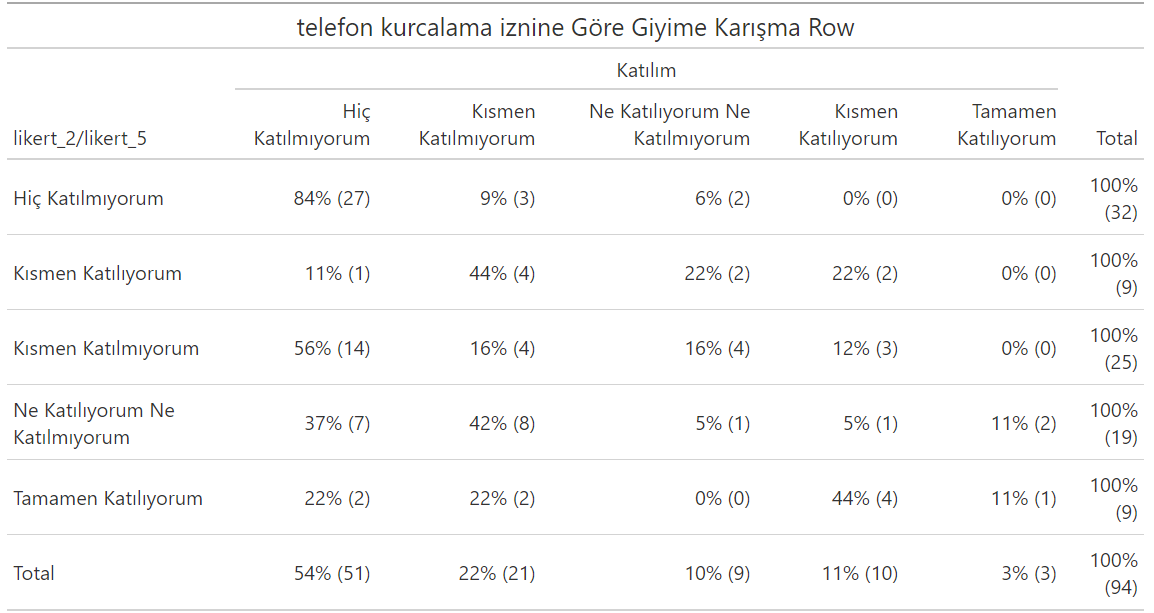
\includegraphics[width=0.8\textwidth]{Imgs/RxC table2.png}
    \label{rxc-table2}
\end{figure}
Tablo \ref{rxc-table2}'den hareketle kız/erkek arkadaşım telefonumu kurcalayabilir sorusuna hiç katılmayan grubun içinde, kız/erkek arkadaşım giyimime karışabilir sorusuna hiç katılmayanların oranı \%84'tür, yorumu yapılmaktadır.

\begin{figure}[htbp]
    \centering
    \caption{RxC Sütun Bazlı Beklenen Frekansları}
    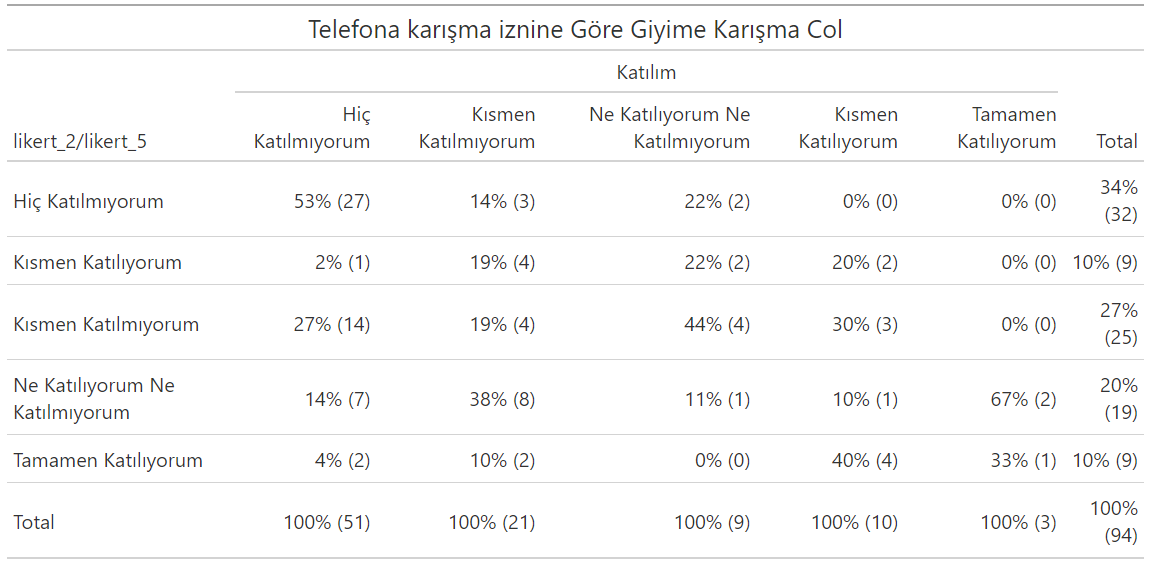
\includegraphics[width=0.8\textwidth]{Imgs/RxC table3.png}
    \label{rxc-table3}
\end{figure}
Tablo \ref{rxc-table3}'den hareketle kız/erkek arkadaşım telefonumu kurcalayabilir sorusuna tamamen katılanların grubu içinde giyime karışılmasına kısment katılanların oranı \%40'tır, yorumu yapılmaktadır.

\begin{verbatim}
       eigenvalue variance.percent cumulative.variance.percent
 Dim.1 0.30406509       62.9669692                    62.96697
 Dim.2 0.09592463       19.8644418                    82.83141
 Dim.3 0.08040571       16.6507242                    99.48214
 Dim.4 0.00250075        0.5178649                   100.00000
\end{verbatim}

Yukarıdaki çıktılardan hareketle aşağıdaki yorumlar yapılmaktadır:
Özdeğerler, her bir eksen tarafından tutulan bilgi miktarına karşılık gelir. Boyutlar azalan şekilde sıralanır ve çözümde açıklanan varyans miktarına göre listelenir. 1. boyut , çözümdeki en fazla varyansı açıklar, ardından boyut 2 sonrasında 3. boyut şeklinde gitmektedir.

`cumulative.variance.percent` kısmını incelediğimizde ilk eksenin \%99.48 oranında açıkladığını görmekteyiz.

Özdeğere alternatif olarak scree-plot grafiklerine de bakılabilir.

\begin{figure}[htbp]
    \centering
    \caption{Scree-Plot}
    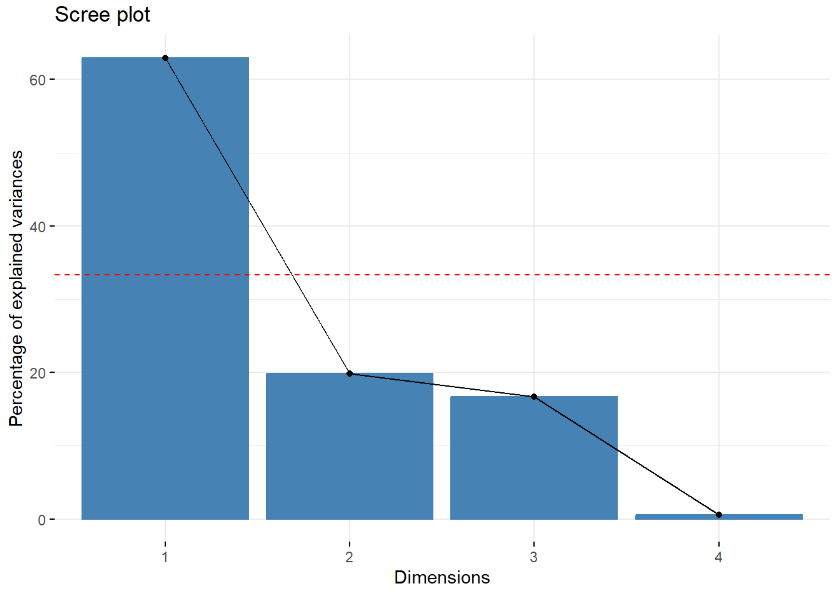
\includegraphics[width=0.5\textwidth]{Imgs/scree-plot.png}
    \label{scree-plot}
\end{figure}
Resim \ref{scree-plot}'ta da görüleceği üzere 4. eksenin toplam varyansı açıklamada etkisiz kalmaktadır. Ancak boyut indirgemesi yaparken ortalam özdeğerin altındakileri çıkarmak üzerine bir yaklaşım yapabiliriz.

Grafiğe göre çözümde sadece 1. boyut kullanılmalıdır. 2. 3. ve 4. boyutlar, ortalama özdeğerin (\%33.33) altında olan toplam inertianın yalnızca yaklaşık \%34’ünü açıklar ve daha fazla analiz için tutulamayacak kadar azdır. (kümülatif değil de ayrı ayrı düşünüldüğünde)

\begin{figure}[htbp]
    \centering
    \caption{CA Bi-Plot}
    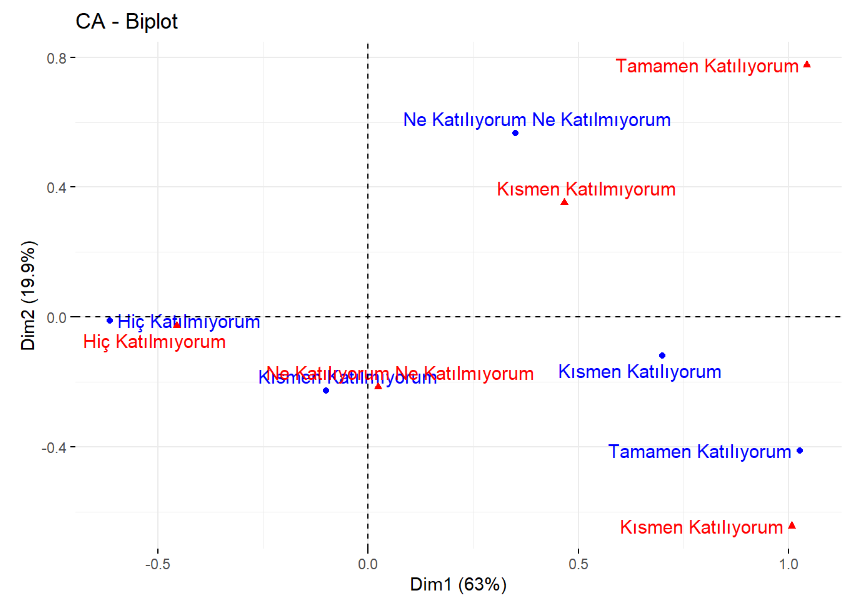
\includegraphics[width=0.5\textwidth]{Imgs/bi-plot.png}
    \label{bi-plot}
\end{figure}

Resim \ref{bi-plot}'ten hareketle;

Mavi noktalar: Satır (telefona karışma izni)

Kırmızı üçgenler: Sütun, değerlerini temsil etmektedir.(giyime karışma izni)

Herhangi bir satır noktası veya sütun noktası arasındaki mesafe, benzerliklerinin (veya benzemezliklerinin) bir ölçüsünü verir.

Grafiğe göre telefonunun kurcalanmasını istemeyen insanların, aynı zamanda giyimlerine de karışılmamasını istemedikleri yorumu yapılabilir. Tam tersi düşünce yapısında da benzer olduğu söylenebilir.

\clearpage
\begin{figure}[htbp]
    \centering
    \caption{Row-Points CA}
    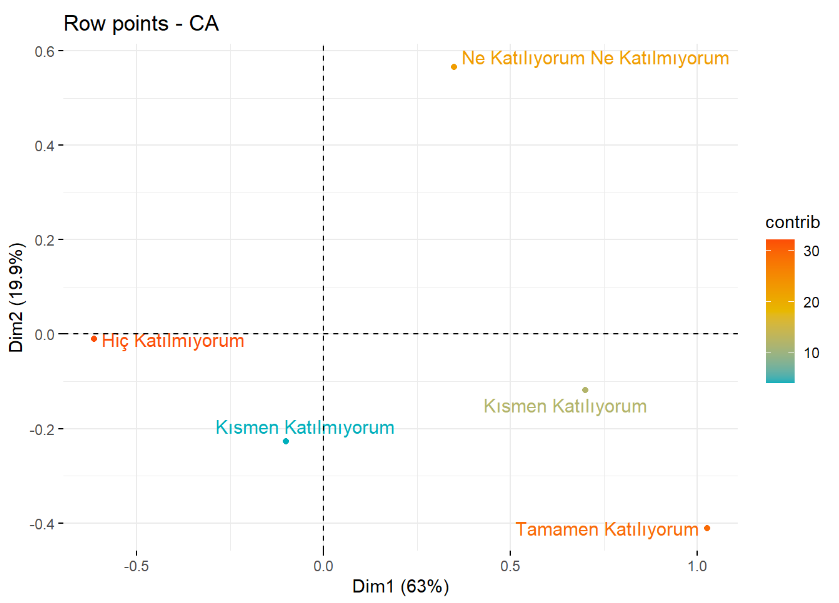
\includegraphics[width=0.5\textwidth]{Imgs/row-points.png}
    \label{row-plot}
\end{figure}

Resim \ref{row-plot}'ten hareketle;
Hiç katılmayanlar ile tamamen katılanlar iki farklı uçta yer almışlardır. Kısmen katılanlar ve tamamen katılanlar ilişkili iken kararsız olanlar farklılık göstermişlerdir.

\begin{figure}[htbp]
    \centering
    \caption{Col-Points CA}
    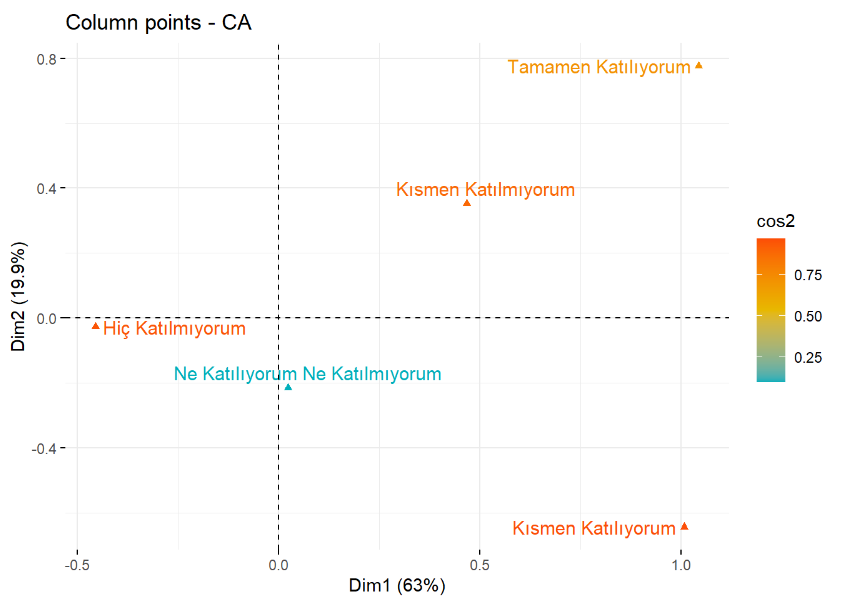
\includegraphics[width=0.5\textwidth]{Imgs/col-points.png}
    \label{col-plot}
\end{figure}

Resim \ref{col-plot}'ten hareketle;
Hiç katılmayanlar ile tamamen katılanlar farklı uçlarda yer almışlardır. Kısmen katılanlar ise farklılık göstermişlerdir.

\clearpage
\subsection{ODDS Oranı}
Çözümleme yapılırken değişkenler aşağıdaki gibi belirlenmiştir:
\begin{enumerate}
    \item \textbf{R (Satır Değişkeni)}: Cinsiyet
    \item \textbf{C (Sütun Değişkeni)}: Soru 10, Kız/Erkek ilişkilerinde başarının anahtarı sizce nedir?
\end{enumerate}
Cinsiyet satır için "Kız/Erkek ilişkilerinde başarının anahtarı sizce nedir?" ise sütun için kabul edilen değişkenlerdir. Çapraz tablo Tablo \ref{tab:relations}'deki gibi elde edilmiştir.
\begin{table}[h]
    \centering
    \caption{RxC Çapraz Tablo Sonuçları}
    \begin{tabular}{|l|c|c|c|}
        \hline
        \multicolumn{1}{|c|}{\textbf{Cinsiyet}} & \multicolumn{3}{c|}{\textbf{Kız/Erkek ilişkilerinde başarı faktörleri}} \\
        \cline{2-4}
        & İletişim Beceleri & Karşılıklı sevgi ve anlayış & Ortak ilgi ve hobiler \\
        \hline
        Erkek & 9 & 21 & 1 \\
        Kadın & 20 & 39 & 4 \\
        \hline
    \end{tabular}
    \label{tab:relations}
\end{table}

ODDS Oranı R programı üzerinde `vcd` kütüphanesi kullanılarak hesaplandı ve çıktı aşağıdaki gibi elde edildi.

\begin{verbatim}
 odds ratios for Sex and soru10 

      A:B       B:C 
0.8357143 2.1538462
\end{verbatim}

Değişkenler çıktıda yer kaplamasın diye harfler ile sembolize edildi:
\begin{itemize}
    \item A: İletişim becerileri
    \item B: Karşılıklı sevgi ve anlayış
    \item C: Ortak ilgi ve hobiler
\end{itemize}

\vspace{10pt}

Çıktılardan hareketle aşağıdaki yorumlar yapıldı:
\begin{itemize}
    \item Erkeklerin kadınlara göre ilişkilerinde başarının anahtarını, karşılıklı sevgi ve anlayış (A) olarak görmesi olasılığı İletişim becerileri (B) olarak görmesi olasılığından 0.8357143 kat azdır.
    \item Kadınların erkeklere göre ilişkilerinde başarının anahtarını, karşılıklı sevgi ve anlayış (A) olarak görmesi olasılığı İletişim becerileri (B) olarak görmesi olasılığından 1.19 (1/0.8357143 = 1.19 ) kat fazladır.
    \item Erkeklerin kadınlara göre ilişkilerinde başarının anahtarını, İletişim becerileri (B) olarak görmesi olasılığı Ortak ilgi ve hobiler (C) olarak görmesi olasılığından 2.1538462 kat fazladır.
\end{itemize}

\textbf{Not:} \\
R dilinde, kategorik değişkenlerin referans kategorileri varsayılan olarak alfabetik veya sayısal olarak en düşük değer olan kategori olarak atanır.
Bu durumda, “Sex” değişkeni “Erkek” ve “Kadın” kategorilerini içeriyor. R, bu durumda “Erkek” kategorisini referans kategorisi olarak kabul eder ve diğer kategorilerle karşılaştırmalar yapar. Dolayısıyla, çıktılarda “Erkek” kategorisi için referans olarak alınır.

Önem kontrolü sonuçları ise aşağıdaki gibi elde edildi:
\begin{verbatim}
                    2.5 %    97.5 %
Erkek:Kadın/A:B 0.3235750  2.158443
Erkek:Kadın/B:C 0.2259705 20.529469    
\end{verbatim}

\[
H_0: \theta_{12} = 1
\]
\[
H_1: \theta_{12} \neq 1
\]
Önem kontrolü sonuçlarından hareketle, güven aralığı 1’i içerdiği için H$_0$ reddedilemez ve $\theta_{12}$’nin istatistiksel olarak anlamlı olmadığı \%95 güvenle söylenebilir.

\[
H_0: \theta_{13} = 1
\]
\[
H_1: \theta_{13} \neq 1
\]
Önem kontrolü sonuçlarından hareketle, güven aralığı 1’i içerdiği için H$_0$ reddedilemez ve $\theta_{13}$’ün istatistiksel olarak anlamlı olmadığı \%95 güvenle söylenebilir.

\vspace{20pt}
\subsection{OxN ve NxO Modelleri}
\subsubsection{NxO Çözümlemesi:} \\
Çözümleme yapılırken satır için cinsiyet değişkeni sütun için ise "Kız/Erkek arkadaşım ben olmadan gece eğlenmeye çıkabilir." önergeli soru alınmıştır.

Likert ölçek sorusu olduğu için "Katılma Düzeyi (1,2,3,4,5)" ordinal değişken olarak kabul edilmiştir.

\begin{verbatim}
    
Likelihood summary table:
         AIC    BIC LR Chisq Df Pr(>Chisq)
model 55.765 57.883   2.8796  3     0.4106
\end{verbatim}

H$_0$: Satır etki modeline uyum vardır. \\
H$_1$: Satır etki modeline uyum yoktur. \\

Yukarıdaki çıktıdan hareketle p-değeri=0.4106, $\alpha$=0.05’ten büyük olduğu için yokluk hipotezi reddedilemez. \%95 Güvenle söylenebilir ki satır etki modeline uyum vardır.

\textbf{Not:} \\
Satır modeline uyum olduğu için, beklenen sıklıklar üzerinden satır düzeyindeki yerel odds oranları birbirine eşittir

\begin{verbatim}

Call:
glm(formula = Frekansı ~ Ölçek + Sex * likertSkor, family = poisson, 
    data = yeni_tablo)

Coefficients: (1 not defined because of singularities)
                Estimate Std. Error z value Pr(>|z|)    
(Intercept)      2.07132    0.11929  17.364  < 2e-16 ***
Ölçek1          -0.13262    0.23949  -0.554 0.579747    
Ölçek2          -0.46598    0.27256  -1.710 0.087328 .  
Ölçek3           0.02398    0.22096   0.109 0.913567    
Ölçek4           0.63605    0.17520   3.630 0.000283 ***
Sex1             0.33104    0.29338   1.128 0.259171    
likertSkor            NA         NA      NA       NA    
Sex1:likertSkor -0.21083    0.08560  -2.463 0.013781 *  
---
Signif. codes:  0 '***' 0.001 '**' 0.01 '*' 0.05 '.' 0.1 ' ' 1

(Dispersion parameter for poisson family taken to be 1)

    Null deviance: 36.7359  on 9  degrees of freedom
Residual deviance:  2.8796  on 3  degrees of freedom
AIC: 55.765

Number of Fisher Scoring iterations: 4
\end{verbatim}

Satır etki modeline göre $\hat{\mu}_1$ katsayısı -0.21083 olarak tahmin edilmiştir. Buradan hareketle \\
$\hat{\mu}_2$=0-(-0.21083)=0.21083 olarak bulunmuş oldu. Satır etkileri için;  

\[
H_0: \mu_{i} = 0
\]
\[
H_1: \mu_{i} \neq 0
\]

p-value=0.013781 < $\alpha$=0.05’ten küçük olduğu için yokluk hipotezi reddedilir. Satır etkisi \%5 hata payıyla istatistiksel olarak anlamlıdır.

\vspace{10pt}
\textbf{Beklenen Sıklıkların Hesaplanması:} \\
Beklenen sıklıklar aşağıdaki gibi elde edildi.
\begin{verbatim}
       Ölçek
Sex     K. Katılmıyorum Katılmıyorum   Nötrüm Katılıyorum K. Katılıyorum
  Erkek        7.837426     6.162574  4.54813    5.451870       6.012566
  Kadın       10.987434     8.980772 25.01923    3.621105      15.378895
\end{verbatim}

\vspace{10pt}
\textbf{ODDS Oranlarının Hesaplanması:} \\
\begin{verbatim}
Sex1:likertSkor 
     -0.2108291 
Sex1:likertSkor 
      0.2108291 
Sex1:likertSkor 
       1.524487 
\end{verbatim}
$$\theta_{11} = e^{\hat{\mu_2} - \hat{\mu_1}} \approx 1.52$$ \\

\textbf{Yorum:} \\
"Kız/Erkek arkadaşım ben olmadan gece eğlenmeye çıkabilir" önergesine katılma durumunun j. düzeyde olanların (j+1). düzeyde olmasına göre, cinsiyetin kadın olmasının erkek olmasına göre bu önergeye katılma olasılığını 1,52 kat arttırmaktadır.

\subsubsection{OxN Çözümlemesi}
Satıra ordinal bir değişken olarak, görüşülen gün sayısı 3 guruba balyalandı. Sütuna ise okunulan bölüm alındı.

\begin{verbatim}
Likelihood summary table:
         AIC    BIC LR Chisq Df Pr(>Chisq)
model 46.562 47.942   3.2757  2     0.1944
\end{verbatim}

$H_0:$ Kurulan sütun etki modele uyum vardır.

$H_1:$ Kurulan sütun etki modele uyum yoktur.  

\vspace{10pt}
p-value=0.1944 değeri $\alpha=0.05$'ten büyük olduğu için yokluk hipotezi reddedilemez. Sütun etki modeline uyum vardır şeklinde bir yorum \%5 hata ile yapılabilir.

\begin{verbatim}
Call:
glm(formula = Freq ~ GörüşülenGün + soru8 * GSkor, family = poisson, 
    data = df_tablo)

Coefficients: (1 not defined because of singularities)
              Estimate Std. Error z value Pr(>|z|)    
(Intercept)     1.3752     0.3139   4.381 1.18e-05 ***
GörüşülenGün1   0.9047     0.3415   2.649  0.00808 ** 
GörüşülenGün2  -0.1631     0.1627  -1.002  0.31627    
soru81         -0.7616     0.6232  -1.222  0.22166    
soru82          0.8373     0.5021   1.667  0.09543 .  
GSkor               NA         NA      NA       NA    
soru81:GSkor    0.2898     0.4074   0.712  0.47677    
soru82:GSkor    0.4864     0.3518   1.383  0.16679    
---
Signif. codes:  0 ‘***’ 0.001 ‘**’ 0.01 ‘*’ 0.05 ‘.’ 0.1 ‘ ’ 1

(Dispersion parameter for poisson family taken to be 1)

    Null deviance: 115.8986  on 8  degrees of freedom
Residual deviance:   3.2757  on 2  degrees of freedom
AIC: 46.562

Number of Fisher Scoring iterations: 5
\end{verbatim}
Satır etki modeline göre $\hat{\tau_1}$ katsayısı 0.2898, $\hat{\tau_2}$ katsayısı 0.4864 olarak tahmin edilmiştir. Buradan hareketle $\hat{\tau_3}=0-(0.2898+0.4864) = -0.7762$ olarak bulunmuş oldu. sütun etkileri için;

$H_0: \tau_i = 0$ 

$H_1: \tau_i \neq 0$

\vspace{10pt}
p-value > $\alpha=0.05$'ten küçük olduğu için yokluk hipotezi reddedilemez. Sütun etkileri istatistiksel olarak anlamlı bulunmamıştır.

\vspace{10pt}
\textbf{ODDS Oranlarının Hesaplanması:} \\
\begin{verbatim}
soru82:GSkor 
    1.217243 
soru81:GSkor 
   0.2828868 
soru81:GSkor 
   0.3443421 
\end{verbatim}
$$\theta_{11} = e^{\hat{\tau_2} - \hat{\tau_1}} \approx 1.22$$ 
$$\theta_{12} = e^{\hat{\tau_3} - \hat{\tau_2}} \approx 0.28$$  
$$\theta_{13} = e^{\hat{\tau_3} - \hat{\tau_1}} \approx 0.34$$  

\textbf{Yorumlar:} \\
\begin{itemize}
    \item "Kız/Erkek arkadaşı seçiminde hangi faktör sizin için en önemlisidir?" sorusuna verilen yanıtlar bakımından "Fizik" yanıtını verenlerin "Karakter" yanıtını verenlere göre Kız/Erkek arkadaşıyla ayda görüştüğü gün sayısının (i+1). düzeyde olmasına göre i. düzeyde olması olasılığı 1.22 kat fazladır.

    \item Kız/Erkek arkadaşıyla ayda görüştüğü gün sayısının (i+1). düzeyde olmasına göre i. düzeyde olanların,"Kız/Erkek arkadaşı seçiminde hangi faktör sizin için en önemlisidir?" sorusuna verdikleri yanıtlar bakımından "Maddiyat" yanıtını vermesi "Karakter" yanıtını vermesine göre ($1/0.28=3.57$) kat fazladır.

    \item Kız/Erkek arkadaşıyla ayda görüştüğü gün sayısının (i+1). düzeyde olmasına göre i. düzeyde olanların,"Kız/Erkek arkadaşı seçiminde hangi faktör sizin için en önemlisidir?" sorusuna verdikleri yanıtlar bakımından "Maddiyat" yanıtını verenlerin "Fizik" yanıtını verenlere göre ($1/0.34=2.94$) kat fazladır.
\end{itemize}

\vspace{20pt}
\subsection{RxCxK Çözümlemesi}
RxCxK çözümlemesi yapılırken aşağıdaki kriterlere göre çözümleme yapılmıştır:
\begin{itemize}
    \item \textbf{R (Satır Değişkeni)}: Likert 1, Kız/Erkek arkadaşımın  sosyal medya kullanımı onun hakkındaki fikirlerimi etkiler.
    \item \textbf{C (Sütun Değişkeni)}: Likert 2, Kız/Erkek arkadaşım telefonumu istediği gibi kurcalayabilir.
    \item \textbf{K (Tabaka Değişkeni)}: Cinsiyet.
\end{itemize}

\vspace{10pt}
\subsubsection{Tam Bağımsızlık (M0) Modeli}
\textbf{Kurulan Model:} [Likert 1][Likert 2][Cinsiyet]

$$H_0: P_{ijk} = P_{i..}P_{.j.}P_{..k}$$

\begin{table}[h]
    \centering
    \caption{Goodness-of-Fit Tests}
    \begin{tabular}{|c|c|c|c|}
         \hline
          & \textbf{Value} & \textbf{df} & \textbf{Sig.} \\
         \hline
         Likelihood Ratio & 67,453 & 40 & 0,004 \\
         Pearson Chi-Square & 69,265 & 40 & 0,003 \\
         \hline
    \end{tabular}
    \label{tab:goodness-of-fit}
\end{table}
Olabilirlik Oran test istatistiği G$^2$=67,453 (p-değeri=0,004) veya Pearson X$^2$ test istatistiği X$^2$=69,265 (p-değeri=0,003) şeklinde bulundu. p-değeri test için belirlenen hata payı $\alpha=0,05$'ten küçük olduğu için H0 reddedilir ve M0 modeline uyum yoktur. Likert 1, Likert 2 ve Cinsiyet değişkenleri arasında \%5 anlamlılık düzeyinde ilişki olduğu söylenmektedir.

\vspace{10pt}
\subsubsection{Kısmi Bağımsızlık (M1) Modeli}
\textbf{Kurulan Model:} [Likert 1][Likert 2 x Cinsiyet];

$$H_0: P_{ijk} = P_{i..}P_{.jk}$$

\begin{table}[h]
    \centering
    \caption{Goodness-of-Fit Tests}
    \begin{tabular}{|c|c|c|c|}
         \hline
          & \textbf{Value} & \textbf{df} & \textbf{Sig.} \\
         \hline
         Likelihood Ratio & 60,448 & 36 & 0,007 \\
         Pearson Chi-Square & 54,465 & 36 & 0,025 \\
         \hline
    \end{tabular}
    \label{tab:goodness-of-fit2}
\end{table}
Olabilirlik Oran test istatistiği G$^2$=60,448 (p-değeri=0,007) veya Pearson X$^2$ test istatistiği X$^2$=54,465 (p-değeri=0,025) şeklinde bulundu. p-değeri test için belirlenen hata payı $\alpha=0,05$'ten küçük olduğu için H0 reddedilir ve M1 modeline uyum yoktur.


\vspace{10pt}
\subsubsection{Kısmi Bağımsızlık (M2) Modeli}
\textbf{Kurulan Model:} [Likert 2] [Likert 1 x Cinsiyet]

$$H_0: P_{ijk} = P_{.j.}P_{i.k}$$

\begin{table}[h]
    \centering
    \caption{Goodness-of-Fit Tests}
    \begin{tabular}{|c|c|c|c|}
         \hline
          & \textbf{Value} & \textbf{df} & \textbf{Sig.} \\
         \hline
         Likelihood Ratio & 41,179 & 24 & 0,016 \\
         Pearson Chi-Square & 33,688 & 24 & 0,090 \\
         \hline
    \end{tabular}
    \label{tab:goodness-of-fit3}
\end{table}
Olabilirlik Oran test istatistiği G$^2$=60,448 (p-değeri=0,007) veya Pearson X$^2$ test istatistiği X$^2$=54,465 (p-değeri=0,025) şeklinde bulundu. Pearson Chi-Square p-değeri test için belirlenen hata payı $\alpha=0,05$'ten büyük olduğu için H0 reddedilemez ve M2 modeline uyum vardır.

\vspace{10pt}
\subsubsection{Kısmi Bağımsızlık (M3) Modeli}
\textbf{Kurulan Model:} [Cinsiyet] [Likert 1 x Likert 2]

$$H_0: P_{ijk} = P_{..k}P_{ij.}$$

\begin{table}[h]
    \centering
    \caption{Goodness-of-Fit Tests}
    \begin{tabular}{|c|c|c|c|}
         \hline
          & \textbf{Value} & \textbf{df} & \textbf{Sig.} \\
         \hline
         Likelihood Ratio & 60,448 & 36 & 0,007 \\
         Pearson Chi-Square & 54,465 & 36 & 0,025 \\
         \hline
    \end{tabular}
    \label{tab:goodness-of-fit4}
\end{table}
Olabilirlik Oran test istatistiği G$^2$=60,448 (p-değeri=0,007) veya Pearson X$^2$ test istatistiği X$^2$=54,465 (p-değeri=0,025) şeklinde bulundu. p-değeri test için belirlenen hata payı $\alpha=0,05$'ten küçük olduğu için H0 reddedilir ve M3 modeline uyum yoktur.

\vspace{10pt}
\subsubsection{Koşullu Bağımsızlık (M4) Modeli}
\textbf{Kurulan Model:} [Likert 1 x Cinsiyet] [Likert 2 x Cinsiyet]

$$H_0: P_{ijk} = P_{i.k}P_{.jk}|P_{..k}$$

\begin{table}[h]
    \centering
    \caption{Goodness-of-Fit Tests}
    \begin{tabular}{|c|c|c|c|}
         \hline
          & \textbf{Value} & \textbf{df} & \textbf{Sig.} \\
         \hline
         Likelihood Ratio & 45,799 & 32 & 0,054 \\
         Pearson Chi-Square & 43,821 & 32 & 0,080 \\
         \hline
    \end{tabular}
    \label{tab:goodness-of-fit5}
\end{table}
Olabilirlik Oran test istatistiği G$^2$=45,799 (p-değeri=0,054) veya Pearson X$^2$ test istatistiği X$^2$=43,821 (p-değeri=0,080) şeklinde bulundu. p-değeri test için belirlenen hata payı $\alpha=0,05$'ten büyük olduğu için H0 reddedilemez ve M4 modeline uyum vardır.

\vspace{10pt}
\subsubsection{Koşullu Bağımsızlık (M5) Modeli}
\textbf{Kurulan Model:} [Likert 1 x Likert 2] [Cinsiyet x Likert 2]

$$H_0: P_{ijk} = P_{ij.}P_{.jk}|P_{.j.}$$

\begin{table}[h]
    \centering
    \caption{Goodness-of-Fit Tests}
    \begin{tabular}{|c|c|c|c|}
         \hline
          & \textbf{Value} & \textbf{df} & \textbf{Sig.} \\
         \hline
         Likelihood Ratio & 34,174 & 20 & 0,025 \\
         Pearson Chi-Square & 25,976 & 20 & 0,167 \\
         \hline
    \end{tabular}
    \label{tab:goodness-of-fit6}
\end{table}
Olabilirlik Oran test istatistiği G$^2$=34,174 (p-değeri=0,025) veya Pearson X$^2$ test istatistiği X$^2$=25,976 (p-değeri=0,167) şeklinde bulundu. p-değeri test için belirlenen hata payı $\alpha=0,05$'ten büyük olduğu için H0 reddedilemez ve M5 modeline uyum vardır.

\vspace{10pt}
\subsubsection{Kısmi Bağımsızlık (M6) Modeli}
\textbf{Kurulan Model:} [Cinsiyet x Likert 1] [Likert 2 x Likert 1]

$$H_0: P_{ijk} = P_{i.k}P_{ij.}|P_{i..}$$

\begin{table}[h]
    \centering
    \caption{Goodness-of-Fit Tests}
    \begin{tabular}{|c|c|c|c|}
         \hline
          & \textbf{Value} & \textbf{df} & \textbf{Sig.} \\
         \hline
         Likelihood Ratio & 26,530 & 20 & 0,149 \\
         Pearson Chi-Square & 21,245 & 20 & 0,383 \\
         \hline
    \end{tabular}
    \label{tab:goodness-of-fit7}
\end{table}
Olabilirlik Oran test istatistiği G$^2$=26,530 (p-değeri=0,149) veya Pearson X$^2$ test istatistiği X$^2$=21,245 (p-değeri=0,383) şeklinde bulundu. p-değeri test için belirlenen hata payı $\alpha=0,05$'ten büyük olduğu için H0 reddedilemez ve M6 modeline uyum vardır.

\vspace{10pt}
\subsubsection{Karşılıklı Bağımsızlık (M7) Modeli}
\textbf{Kurulan Model:} [Cinsiyet x Likert 1] [Likert 2 x Likert 1] [Cinsiyet x Likert 2]

$$H_0: P_{ijk} = P_{ij.}P_{i.k}|P_{.jk}$$

\begin{table}[h]
    \centering
    \caption{Goodness-of-Fit Tests}
    \begin{tabular}{|c|c|c|c|}
         \hline
          & \textbf{Value} & \textbf{df} & \textbf{Sig.} \\
         \hline
         Likelihood Ratio & 22,185 & 16 & 0,137 \\
         Pearson Chi-Square & 18,597 & 16 & 0,290 \\
         \hline
    \end{tabular}
    \label{tab:goodness-of-fit8}
\end{table}
Olabilirlik Oran test istatistiği G$^2$=22,185 (p-değeri=0,137) veya Pearson X$^2$ test istatistiği X$^2$=18,597 (p-değeri=0,290) şeklinde bulundu. p-değeri test için belirlenen hata payı $\alpha=0,05$'ten büyük olduğu için H0 reddedilemez ve M7 modeline uyum vardır.

\vspace{10pt}
Uyum gösteren tüm modeller en iyi modelin belirlenmesi için analiz edildi. AIC ve BIC değerleri Tablo \ref{tab:model-değerlendirme}'deki gibi elde edildi.


\begin{table}[h]
    \centering
    \caption{Model Değerlendirme Sonuçları}
    \begin{tabular}{|c|c|c|}
         \hline
         \textbf{Model}& \textbf{AIC} & \textbf{BIC} \\
         \hline
         M2 & -10,821 & 27,564 \\ 
         M4 & -18,201 & 22,184 \\ 
         M5 & -5,826 & 10,559 \\ 
         M6 & -13,47 & 3,915 \\ 
         M7 & -9,815 & -0,43 \\  
         \hline
    \end{tabular}
    \label{tab:model-değerlendirme}
\end{table}

Tablo \ref{tab:model-değerlendirme}'den hareketle en iyi modelin M4 modeli olduğu söylenmektedir.

\clearpage
\subsection{ NxNxO, NxOxO ve OxOxO Modelleri}
\vspace{10pt}
\textbf{NxOxO Modeli}

\vspace{10pt}
SPSS programında RxCxK tablosunu oluşturabilmek için likert soruları ve yaşanan en uzun ilişki süresi 2 seçeneğe indirgenmiştir. Buna göre;
Likert ölçek sorusundaki, 1,2,3 değerleri 0 (az) olarak 4 ve 5 değerleri 1(çok) olarak güncellenmiştir.
Yaşanan en uzun ilişki süresi (ay) 11 den küçük olanlar 0 (az) olarak, 11 den büyük olanlar 1 (çok) olarak güncellenmiştir. 

\vspace{10pt}
Bu işlemler SPSS üzerinde “Transform > Optimal Binning” üzerinden gerçekleştirilmiştir. \\

\noindent\textbf{R:} Cinsiyet (Kız-Erkek)\\
\textbf{C:} Kız/erkek arkadaşın daha önce yaşadığı ilişkilerin önemli olup olmaması.\\
\textbf{K:} Yaşanan en uzun ilişki süresi. (ay)\\

Tablolar SPSS üzerinde "Analyze > Descriptive Statistics > Crosstabs" kısmından görseldeki gibi oluşturulmuştur. "Statistics" Kısmında "Risk" ve "Cochran's and Mantel-Haenszel statistics" kısmı seçilmiştir.\\

\begin{figure}[h!t]
    \centering
    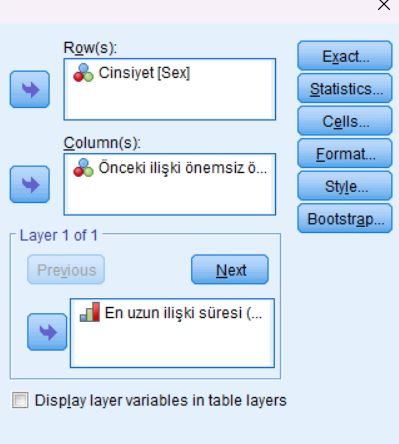
\includegraphics[width=0.5\linewidth]{Imgs/spss_crosstab.jpg}
    \caption{SPSS crosstab sekmesi}
    \label{fig:enter-label}
\end{figure}

\vspace{10pt}
\subsubsection{En Uzun İlişki Süresi Düzeyinde Odds Oranları}
\begin{table}[htbp]
\centering
\caption{Risk Estimate}
\label{tab:risk-estimate}
\begin{tabular}{lccccc}
\hline
\textbf{İlişki Süresi (ay)} & \textbf{Value} & \textbf{Lower} & \textbf{Upper} & \textbf{N of Valid Cases} \\
\hline
\textbf{Az} & & & & \\
Odds Ratio for Cinsiyet (Erkek / Kadın) & 3.200 & 0.919 & 11.145 & 49 \\
For cohort Önceki ilişki önemsiz önemli = Önemsiz & 1.579 & 0.989 & 2.520 & \\
For cohort Önceki ilişki önemsiz önemli = Önemli & 0.493 & 0.217 & 1.124 & \\
\hline
\textbf{Çok} & & & & \\
Odds Ratio for Cinsiyet (Erkek / Kadın) & 1.032 & 0.270 & 3.937 & 45 \\
For cohort Önceki ilişki önemsiz önemli = Önemsiz & 1.013 & 0.578 & 1.775 & \\
For cohort Önceki ilişki önemsiz önemli = Önemli & 0.982 & 0.451 & 2.139 & \\
\hline
\textbf{Total} & & & & \\
Odds Ratio for Cinsiyet (Erkek / Kadın) & 1.909 & 0.776 & 4.700 & 94 \\
For cohort Önceki ilişki önemsiz önemli = Önemsiz & 1.293 & 0.922 & 1.814 & \\
For cohort Önceki ilişki önemsiz önemli = Önemli & 0.677 & 0.382 & 1.200 & \\
\hline
\end{tabular}
\end{table}

\vspace{10pt}
İlişki süresi az olanların, önceki ilişkilerin önemsiz olduğunu düşünme olasılığı, erkeklerde kadınlara göre 3.2 kat daha fazladır. Odds oranının 95\% güven aralığı [0,919;  11,145], “1”i içerdiğinden odds oranının anlamlı olmadığı söylenebilir.

\vspace{10pt}
İlişki süresi çok olanların, önceki ilişkilerin önemsiz olduğunu düşünme olasılığı, erkeklerde, kadınlara göre 1,032 kat daha fazladır . Buradan, ilişki süresi çok olan erkek ve kadınların benzer düşündüğü yorumu yapılabilir. Odds oranının 95\% güven aralığı [0,270;  3,937] “1”i içerdiğinden odds oranının anlamlı olmadığı söylenebilir.

\subsubsection{Breslow Day Testi}

\vspace{50pt}

$$H_0: \theta_{RC1} = \theta_{RC2} $$  

\begin{center}
(en uzun ilişki süresi düzeyinde odds oranları eşittir.)
\end{center}
\vspace{20pt}
\begin{table}[htbp]
\centering
\caption{Tests of Homogeneity of the Odds Ratio}
\label{tab:homogeneity-tests}
\begin{tabular}{lccc}
\hline
 & \textbf{Chi-Squared} & \textbf{df} & \textbf{Asymptotic Significance (2-sided)} \\
\hline
Breslow-Day & 1.487 & 1 & 0.223 \\
Tarone's & 1.486 & 1 & 0.223 \\
\hline
\end{tabular}
\end{table}





\vspace{10pt}
Breslow Day testine ait $\chi^2_{BD}$ istatistiğine göre yokluk hipotezi reddedilemez. (p>0.05) en uzun ilişki süresi üzerinden hesaplanan odds oranları homojendir. 

\subsubsection{Ortak Odds Oranları}

\begin{center}
    $H_0:$ Ortak odds oranı önemsizdir.  
\end{center}

\begin{table}[htbp]
\centering
\caption{Tests of Conditional Independence}
\label{tab:conditional-independence-tests}
\begin{tabular}{lccc}
\hline
 & \textbf{Chi-Squared} & \textbf{df} & \textbf{Asymptotic Significance (2-sided)} \\
\hline
Cochran's & 2.062 & 1 & 0.151 \\
Mantel-Haenszel & 1.438 & 1 & 0.230 \\
\hline
\end{tabular}
\end{table}

Under the conditional independence assumption, Cochran's statistic is asymptotically distributed as a 1 df chi-squared distribution, only if the number of strata is fixed, while the Mantel-Haenszel statistic is always asymptotically distributed as a 1 df chi-squared distribution. Note that the continuity correction is removed from the Mantel-Haenszel statistic when the sum of the differences between the observed and the expected is 0.

\vspace{20pt}
Mantel-Haenszel test istatistiklerine göre yokluk hipotezi reddedilemez. p>0.05. Ortak odds oranının önemsiz olduğu 95\% güven düzeyinde söylenebilir. 

\vspace{20pt}
\begin{table}[htbp]
\centering
\caption{Mantel-Haenszel Common Odds Ratio Estimate}
\label{tab:mantel-haenszel-estimate}
\begin{tabular}{lcc}
\hline
\textbf{Estimate} & 1,907 \\
\textbf{ln(Estimate)} & 0.645 \\
\textbf{Standard Error of ln(Estimate)} & 0.457 \\
\textbf{Asymptotic Significance (2-sided)} & 0.158 \\
\hline
\multicolumn{3}{l}{\textbf{Asymptotic 95\% Confidence Interval}} \\
Common Odds Ratio & Lower Bound & 0.778 \\
 & Upper Bound & 4.674 \\
ln(Common Odds Ratio) & Lower Bound & -0.251 \\
 & Upper Bound & 1.542 \\
\hline
\end{tabular}
\end{table}

The Mantel-Haenszel common odds ratio estimate is asymptotically normally distributed under the common odds ratio of 1.000 assumption. So is the natural log of the estimate.

$$H_0: \hat{\theta}_{\text{MH}} = 1$$
Ortak odds oranı $\hat{\theta}_{\text{MH}}$ = 1.907 dir. Ancak yukarıda belirtildiği üzere anlamlı değildir. Bu yüzden diğer istatistikleri yorumlamaya gerek yoktur.



\clearpage
\section{Kaynakça}
\begin{enumerate}
    \item \href{https://www.hacettepe.edu.tr/ogretim/sayilarla_ogretim}{Hacettepe Üniversitesi fakülte bazlı numerik genel bilgiler}
    \item \href{https://stat.hacettepe.edu.tr/tr/menu/ogretim_uyeleri-118}{Hacettepe Üniversitesi İstatistik Bölümü akademik personel verileri}
    \item \href{https://aktuerya.hacettepe.edu.tr/pers_ou.php}{Hacettepe Üniversitesi Aktüerya Bölümü akademik personel verileri}
    \item \href{https://mat.hacettepe.edu.tr/akademik_personel.html}{Hacettepe Üniversitesi Matematik Bölümü akademik personel verileri}
    \item \href{https://chem.hacettepe.edu.tr/tr/menu/ogretim_uyeleri-10}{Hacettepe Üniversitesi Kimya Bölümü akademik personel verileri}
    \item \href{https://biology.hacettepe.edu.tr/tr/akademik_personel-226}{Hacettepe Üniversitesi Biyoloji Bölümü akademik personel verileri}
    \item \href{https://www.statology.org}{Statology}
    \item \href{https://docs.google.com/forms/d/e/1FAIpQLSf7CBA1tg89lFSdAl9VRSa4vjmv8COCJtRDvQmYa0n0l72JUA/viewform?usp=sf_link}{Form Bağlantısı} \label{form}
\end{enumerate}

\end{document}

